\twocolumn[\colorsection{Distribuciones de carga contínuas}]
\setcounter{figure}{0}

\begin{Exercise}
  Un alambre recto, muy largo, tiene una densidad de carga por unidad de longitud $\lambda = \SI{1.46}{\nano\coulomb/\metre}$. ¿A qué distancia desde el alambre la magnitud del campo eléctrico es $\SI{25.0}{\newton/\coulomb}$?
\end{Exercise}
\begin{Answer}
  $\SI{1.05}{\metre}$
\end{Answer}
%
\begin{Exercise}\label{p:continuas01}
  \textbf{\raisebox{.5pt}{\textcircled{\raisebox{-1.2pt} {E}}}} \textit{a}) Para el segmento mostrado en la figura \ref{f:continuas01}, de longitud $L$ y carga $Q$ distribuida uniformemente, demuestre que el campo eléctrico en el punto $S$ ubicado a una distancia $a$ sobre la mediatriz, está dado por:
  \begin{align*}
    \va*{E} &= \frac{Q}{2\pi\varepsilon_o a} \frac{1}{\sqrt{L^2+4a^2}}\vu{y}
  \end{align*}
  \textit{b}) Para el mismo segmento, demuestre que el campo eléctrico en el punto $P$ vale:
  \begin{align*}
    \va*{E} = \frac{Q}{4\pi\varepsilon_o L} \left \lbrack \frac{1}{b} - \frac{1}{L+b} \right \rbrack \vu{x}
  \end{align*}
  \textit{c}) Si la longitud del segmento es $L = \SI{5.0}{\centi\metre}$ y su carga es $Q = \SI{1.0}{\micro\coulomb}$, calcular la fuerza sobre una carga puntual de $\SI{3.0}{\micro\coulomb}$ si se la ubica en el punto $P$, a una distancia $b = \SI{2.0}{\centi\metre}$.
\end{Exercise}
\begin{Answer}
  \textit{c}) $\va*{F} = \SI{19.3}{\newton}\vu{x}$
\end{Answer}
%
\begin{center}
\begin{tikzpicture}[scale=0.4]
  \draw (0,0) ellipse (0.1 and 0.2);
  \draw (-5,0) +(90:0.1 and 0.2) arc (90:270:0.1 and 0.2);
  \draw [black] (-5,0.2)--(0,0.2);
  \draw [black] (-5,-0.2)--(0,-0.2);
  \draw [blue, dotted] (0,0)--(5,0);
  \draw [blue, dotted] (-7,0)--(-5.1,0);
  \draw [blue, dotted] (-2.5,0.2)--(-2.5,4);
  \draw [blue, dotted] (-2.5,-0.2)--(-2.5,-2);
  \draw [black, -{Stealth}] (-12,0)--(-8,0) node[below] {$x$};
  \draw [black, -{Stealth}] (-11,-1)--(-11,3.5) node[left] {$y$};
  \draw [blue, {Stealth}-{Stealth}] (-3.5,0.2)--(-3.5,3) node[midway, left] {$a$};
  \draw [blue, {Stealth}-{Stealth}] (0,-1)--(4,-1) node[midway, above] {$b$};
  \fill [blue](4,0) circle(5pt) node[above right] {$P$};
  \fill [blue](-2.5,3) circle(5pt) node[above right] {$S$};
\end{tikzpicture}
\captionof{figure}{Problema \ref{p:continuas01}\label{f:continuas01}}
\end{center}
%
\begin{Exercise}\label{p:continuas02}
  \textbf{\raisebox{.5pt}{\textcircled{\raisebox{-1.2pt} {E}}}} Dos varillas delgadas de longitud $L = \SI{3.00}{\centi\metre}$ están a lo largo del eje $x$ como se muestra en la figura \ref{f:continuas02}. Cada varilla tiene carga igual a $\SI{5.00}{\micro\coulomb}$ distribuida de manera uniforme en toda su longitud. Calcular el módulo de la fuerza que ejerce una varilla sobre la otra.
\end{Exercise}
\begin{Answer}
  $\SI{50.7}{\newton}$
\end{Answer}
%
\begin{center}
  \begin{tikzpicture}[scale=0.5]
    \draw (5,0) ellipse (0.1 and 0.2);
    \draw (2,0) +(90:0.1 and 0.2) arc (90:270:0.1 and 0.2);
    \draw [black] (2,0.2)--(5,0.2);
    \draw [black] (2,-0.2)--(5,-0.2);
    \draw (-2,0) ellipse (0.1 and 0.2);
    \draw (-5,0) +(90:0.1 and 0.2) arc (90:270:0.1 and 0.2);
    \draw [black] (-5,-0.2)--(-2,-0.2);
    \draw [black] (-5,0.2)--(-2,0.2);
    \draw [blue, dotted, -{Stealth}] (-7,-0.7)--(7,-0.7) node[below] {$x$};
    \draw [blue] (-5,-0.5)--(-5,-0.9) node[below] {$-5$};
    \draw [blue] (-2,-0.5)--(-2,-0.9) node[below] {$-2$};
    \draw [blue] (0,-0.5)--(0,-0.9) node[below] {$0$};
    \draw [blue] (2,-0.5)--(2,-0.9) node[below] {$2$};
    \draw [blue] (5,-0.5)--(5,-0.9) node[below] {$5$};
  \end{tikzpicture}
  \captionof{figure}{Problema \ref{p:continuas02}\label{f:continuas02}}
\end{center}
%
\begin{Exercise}\label{p:continuas03}
Se tienen dos hilos infinitos con densidad lineal de carga uniforme, ubicados como muestra la figura \ref{f:continuas03}. Uno de los hilos se prolonga a lo largo del eje $y$ ($x=0$) y tiene densidad de carga $\lambda_1 = \SI{-30}{\micro\coulomb/\metre}$, y el otro hilo se encuentra a una distancia $b = \SI{20}{\centi\metre}$ medida sobre el eje $x$, y su densidad de carga es $\lambda_2 = \SI{10}{\micro\coulomb/\metre}$. ¿En qué posiciones sobre el eje $x$ se puede ubicar una carga puntual positiva si se desea que la fuerza neta sobre dicha carga esté dirigida hacia el sentido positivo de $x$?
\end{Exercise}
\begin{Answer}
  \begin{minipage}[t]{.4\textwidth}
  La carga puede estar en $ x < \SI{0}{\centi\metre}$, en $\SI{15}{\centi\metre} < x < \SI{20}{\centi\metre}$,\\ o en $\SI{20}{\centi\metre} < x < \SI{30}{\centi\metre}$
  \end{minipage}
\end{Answer}
%
\begin{center}
  \begin{tikzpicture}[scale=0.5]
    \draw (0,3.5) ellipse (0.2 and 0.1);
    \draw (0,-1.5) +(180:0.2 and 0.1) arc (180:360:0.2 and 0.1);
    \draw [black] (-0.2,-1.5)--(-0.2,3.5) node[midway, left] {$\lambda_1$};
    \draw [black] (0.2,-1.5)--(0.2,3.5);
    \draw (2,3.5) ellipse (0.2 and 0.1);
    \draw (2,-1.5) +(180:0.2 and 0.1) arc (180:360:0.2 and 0.1);
    \draw [black] (1.8,-1.5)--(1.8,3.5);
    \draw [black] (2.2,-1.5)--(2.2,3.5) node[midway, right] {$\lambda_2$};
    \draw [blue, -{latex}] (2.2,0)--(5,0) node[below] {$x$};
    \draw [blue] (0.2,0)--(1.8,0);
    \draw [blue] (-2,0)--(-0.2,0);
    \draw [blue, -{latex}] (0,3.5)--(0,4.5) node[left] {$y$};
    \draw [blue] (0,-2.5)--(0,-1.6);
    \draw [blue, {latex}-{latex}] (0.05,-2)--(1.95,-2) node[midway, above] {$b$};
  \end{tikzpicture}
  \captionof{figure}{Problema \ref{p:continuas03}\label{f:continuas03}}
\end{center}
%
\begin{Exercise}
  Verifique que la diferencia de potencial eléctrico entre dos puntos situados a distancias $a$ y $b$ de un hilo infinito, con densidad de carga uniforme $\lambda$, es:
  \begin{flalign*}
    V_b - V_a &= \dfrac{\lambda}{2\pi \varepsilon_0} \ln{\dfrac{a}{b}}
  \end{flalign*}
\end{Exercise}
%
\begin{Exercise}\label{p:potencial05}
  La figura \ref{f:potencial05} muestra un hilo infinito que se prolonga a lo largo del eje $y$ ($x=0$), con densidad de carga $\lambda_1 = \SI{-300}{\nano\coulomb/\metre}$, y otro hilo paralelo al primero que pasa por $x = \SI{20}{\centi\metre}$, con densidad de carga $\lambda_2 = \SI{100}{\nano\coulomb/\metre}$. Los puntos $A$, $B$ y $C$ están en las posiciones $x_A = \SI{-10}{\centi\metre}$, $x_B = \SI{10}{\centi\metre}$ y $x_C = \SI{30}{\centi\metre}$. Calcule las siguientes diferencias de potencial eléctrico: \textit{a}) $V_B-V_A$, \textit{b}) $V_C-V_B$, \textit{c}) $V_C-V_A$.
\end{Exercise}
\begin{Answer}
  \begin{minipage}[t]{.4\textwidth}
    \textit{a}) $\SI{1980}{\volt}$\\ \textit{b}) $\SI{5930}{\volt}$\\ \textit{c}) $\SI{7910}{\volt}$
  \end{minipage}
\end{Answer}
%
\begin{center}
  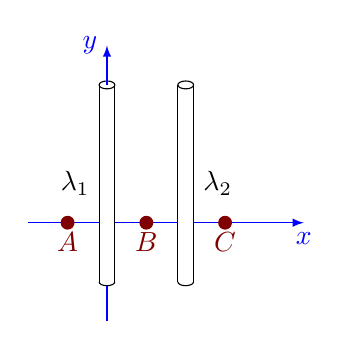
\begin{tikzpicture}[scale=0.5]
    \draw (0,3.5) ellipse (0.2 and 0.1);
    \draw (0,-1.5) +(180:0.2 and 0.1) arc (180:360:0.2 and 0.1);
    \draw [black] (-0.2,-1.5)--(-0.2,3.5) node[midway, left] {$\lambda_1$};
    \draw [black] (0.2,-1.5)--(0.2,3.5);
    \draw (2,3.5) ellipse (0.2 and 0.1);
    \draw (2,-1.5) +(180:0.2 and 0.1) arc (180:360:0.2 and 0.1);
    \draw [black] (1.8,-1.5)--(1.8,3.5);
    \draw [black] (2.2,-1.5)--(2.2,3.5) node[midway, right] {$\lambda_2$};
    \draw [blue, -{latex}] (2.2,0)--(5,0) node[below] {$x$};
    \draw [blue] (0.2,0)--(1.8,0);
    \draw [blue] (-2,0)--(-0.2,0);
    \draw [blue, -{latex}] (0,3.5)--(0,4.5) node[left] {$y$};
    \draw [blue] (0,-2.5)--(0,-1.6);
    \fill [red!50!black](-1,0) circle(5pt) node[below] {$A$};
    \fill [red!50!black](1,0) circle(5pt) node[below] {$B$};
    \fill [red!50!black](3,0) circle(5pt) node[below] {$C$};
  \end{tikzpicture}
  \captionof{figure}{Problema \ref{p:potencial05}\label{f:potencial05}}
\end{center}
%
\begin{Exercise}
  Calcular la energía cinética de un electrón que gira en una trayectoria circular alrededor de un hilo infinito con densidad de carga $\lambda = \SI{3E-8}{\coulomb/\metre}$.
\end{Exercise}
\begin{Answer}
  $\SI{4.32E-17}{\joule}$
\end{Answer}
%
\begin{Exercise}\label{p:potencial06}
  \textbf{\raisebox{.5pt}{\textcircled{\raisebox{-1.2pt} {E}}}} Para la barra mostrada en la figura \ref{f:potencial06}, con densidad lineal de carga $\lambda$: \textit{a}) Verifique que el potencial eléctrico en el punto $P$ es:
  \begin{flalign*}
    V_P &= \frac{\lambda}{4 \pi \varepsilon_o} \ln \left ( \frac{a-L/2}{a+L/2} \right )
  \end{flalign*}
  b) Compruebe que en el caso $a \gg L$ se puede aproximar por:
  \begin{flalign*}
    V_P &\approx \frac{\lambda}{4 \pi \varepsilon_o} \frac{L}{a}
  \end{flalign*}
\end{Exercise}
%
\begin{center}
  \begin{tikzpicture}[scale=0.5]
    \draw (0,0) ellipse (0.1 and 0.2);
    \draw (-5,0) +(90:0.1 and 0.2) arc (90:270:0.1 and 0.2);
    \draw [black] (-5,0.2)--(0,0.2);
    \draw [black] (-5,-0.2)--(0,-0.2);
    \draw [blue, dotted] (0,0)--(5,0);
    \draw [blue, dotted] (-7,0)--(-5.1,0);
    % \draw [blue, dotted] (-2.5,0.2)--(-2.5,4);
    \draw [blue, dotted] (-2.5,-0.2)--(-2.5,-2);
    % \draw [black, -{Stealth}] (-12,0)--(-8,0) node[below] {$x$};
    % \draw [black, -{Stealth}] (-11,-1)--(-11,3.5) node[left] {$y$};
    \draw [blue, {Stealth}-{Stealth}] (-5,1)--(0,1) node[midway, above] {$L$};
    \draw [blue, {Stealth}-{Stealth}] (-2.5,-1)--(3,-1) node[midway, below] {$a$};
    \fill [blue](3,0) circle(5pt) node[above right] {$P$};
    % \fill [blue](-2.5,3) circle(5pt) node[above right] {$S$};
  \end{tikzpicture}
  \captionof{figure}{Problema \ref{p:potencial06}\label{f:potencial06}}
\end{center}
%
\begin{Exercise}\label{p:continuas04}
  \textbf{\raisebox{.5pt}{\textcircled{\raisebox{-1.2pt} {E}}}} \textit{a}) Para el disco mostrado en la figura \ref{f:continuas04}, cuyo radio es $R$ y está cargado con una densidad de carga superficial $\sigma$ uniforme, demuestre que el campo eléctrico producido en el punto $P$ es:
  \begin{align*}
    \va*{E} &= \frac{\sigma}{2\varepsilon_o} \left [ 1 - \frac{z}{\sqrt{z^2+R^2}} \right ] \vu{k}
  \end{align*}
  \textit{b}) Sea la carga neta que se distribuye uniformemente en la superficie del disco igual a $\SI{-6.50}{\nano\coulomb}$ y su radio $R = \SI{1.25}{\centi\metre}$, calcular el campo eléctrico que produce este disco en el punto $P$ a una distancia $z = \SI{2.00}{\centi\metre}$ desde su centro. \textit{c}) Con los mismos valores del ítem \textit{b}, calcular el campo eléctrico en el punto $P$ suponiendo que toda la carga se distribuyera uniformemente en el perímetro del disco.
\end{Exercise}
\begin{Answer}
  \begin{minipage}[t]{.4\textwidth}
    \textit{b}) $\va*{E} = \SI{-1.14E5}{\newton/\coulomb}\vu{k}$\\ \textit{c}) $\va*{E} = \SI{-8.91E4}{\newton/\coulomb}\vu{k}$
  \end{minipage}
\end{Answer}
%
\begin{center}
  \tdplotsetmaincoords{70}{110}
  \begin{tikzpicture}[tdplot_main_coords, scale=0.5]
    %Axis
    \filldraw[fill=red, opacity=0.2,tdplot_main_coords] (4,0,0) arc (0:360:4);
    \draw[axis] (0,0,0) -- (6,0,0) node [pos=1.1] {$i$};
    \draw[axis] (0,0,0) -- (0,6,0) node [pos=1.05] {$j$};
    \draw[axis] (0,0,0) -- (0,0,5.5)  node [left] {$k$};
    \fill [black](0,0,4) circle(3pt) node[left] {$P = (0,0,z)$};
  \end{tikzpicture}
  \captionof{figure}{Problema \ref{p:continuas04}\label{f:continuas04}}
\end{center}
%
\begin{Exercise}\label{p:continuas05}
  El anillo mostrado en la figura \ref{f:continuas05} tiene un radio de $\SI{2.50}{\centi\metre}$ y una carga total igual $\SI{0.125}{\nano\coulomb}$ distribuida uniformemente. El centro del anillo está en el origen de coordenadas. Una carga puntual $q = \SI{-2.50}{\micro\coulomb}$ se coloca sobre el eje $k$ a una altura $b = \SI{40.0}{\centi\metre}$. ¿Cuál es la fuerza ejercida sobre el anillo debida a la carga $q$?
\end{Exercise}
\begin{Answer}
  $\va*{F} = \SI{1.74E-5}{\newton}\vu{k}$
\end{Answer}
%
\begin{center}
  \tdplotsetmaincoords{70}{110}
  \begin{tikzpicture}[tdplot_main_coords, scale=0.5]
    %Axis
    \draw[thick, tdplot_main_coords] (4,0,0) arc (0:360:4);
    \draw[axis] (0,0,0) -- (6,0,0) node [pos=1.1] {$i$};
    \draw[axis] (0,0,0) -- (0,6,0) node [pos=1.05] {$j$};
    \draw[axis] (0,0,0) -- (0,0,5.5)  node [left] {$k$};
    \fill [black](0,0,4) circle(4pt) node[right] {$q$};
    \draw[blue, {Stealth}-{Stealth}] (0.5,-0.5,0) -- (0.5,-0.5,4) node[midway, left] {$b$};
  \end{tikzpicture}
  \captionof{figure}{Problema \ref{p:continuas05}\label{f:continuas05}}
\end{center}
%
\begin{Exercise}\label{p:continuas06}
  \textbf{\raisebox{.5pt}{\textcircled{\raisebox{-1.2pt} {E}}}} \textit{a}) Una carga de $\SI{-12.0}{\nano\coulomb}$ está distribuida de manera uniforme en un cuarto de círculo de radio $a = \SI{25.0}{\centi\metre}$ que se encuentra en el primer cuadrante, con el centro de curvatura en el origen, como se muestra en la figura \ref{f:continuas06}. Calcular el campo eléctrico en el origen. \textit{b}) Encontrar el campo eléctrico en el centro de la semicircunferencia de radio $R$ y densidad de carga lineal uniforme $\lambda$ mostrada en la figura \ref{f:continuas07}.
\end{Exercise}
\begin{Answer}
  \begin{minipage}[t]{.4\textwidth}
    \textit{a}) $|\va*{E}| = \SI{432}{\newton/\coulomb}$; $\theta = 45^\circ$\\ \textit{b}) $\va*{E} = \dfrac{\lambda}{2\pi\varepsilon_o R}\vu{x}$
  \end{minipage}
\end{Answer}
%
\begin{center}
  \begin{tikzpicture}[scale=0.6]
    \draw [very thick] (3,0) arc (0:90:3);
    \draw [blue, -{latex}] (0,0)--(2.12,2.12) node[midway, above] {$a$};
    \draw [blue, -{latex}] (0,-2)--(0,4) node[left] {$y$};
    \draw [blue, -{latex}] (-2,0)--(4,0) node[below] {$x$};
  \end{tikzpicture}
  \captionof{figure}{Problema \ref{p:continuas06} (\textit{a})\label{f:continuas06}}
\end{center}
%
\begin{center}
  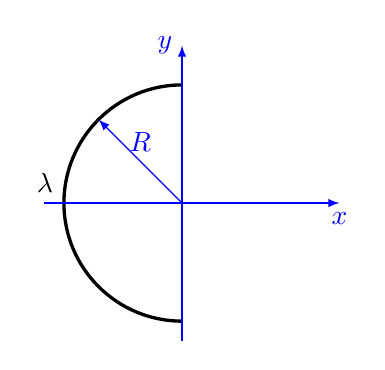
\begin{tikzpicture}[scale=0.5]
    \draw [very thick] (0,3) arc (90:270:3) node[midway, above left] {$\lambda$};
    \draw [blue, -{latex}] (0,0)--(-2.12,2.12) node[midway, above] {$R$};
    \draw [blue, -{latex}] (0,-3.5)--(0,4) node[left] {$y$};
    \draw [blue, -{latex}] (-3.5,0)--(4,0) node[below] {$x$};
  \end{tikzpicture}
  \captionof{figure}{Problema \ref{p:continuas06} (\textit{b})\label{f:continuas07}}
\end{center}
%
%
\begin{Exercise}
  \textbf{\raisebox{.5pt}{\textcircled{\raisebox{-1.2pt} {E}}}} Considere una espira circular de radio $R$, cargada con densidad lineal de carga uniforme $\lambda$. \textit{a}) Verifique que el potencial eléctrico en un punto $P$ situado a una altura $z$ del eje de la espira es:
  \begin{flalign*}
    V_P &= \dfrac{R\lambda}{2\varepsilon_o\sqrt{R^2+z^2}}
  \end{flalign*}
  \textit{b}) Verifique el resultado del campo eléctrico en ese punto obteniendo el gradiente del potencial.
\end{Exercise}
%
\begin{Exercise}
  \textbf{\raisebox{.5pt}{\textcircled{\raisebox{-1.2pt} {E}}}} Verifique que el potencial en un punto $P$ sobre el eje de un disco plano, a una distancia $z$ del centro del mismo, si el radio del disco es $R$ y la densidad superficial de carga es $\sigma$ es:
  \begin{flalign*}
    V_P &= \dfrac{\sigma}{2\varepsilon_o} \left ( \sqrt{R^2+Z^2} - Z \right )
  \end{flalign*}
\end{Exercise}
%
\begin{Exercise}\label{p:continuas08}
  Sean dos planos paralelos al plano $yz$, cargados con igual densidad de carga uniforme $\sigma$ y separados por una distancia $a$ como se muestra en la figura \ref{f:continuas08}. Obtener el campo eléctrico en las regiones $x<0$, $0<x<a$ y $a<x$, para puntos alejados de los bordes y cuya distancia al plano sea pequeña comparada con las dimensiones de los planos.
\end{Exercise}
\begin{Answer}
  \begin{minipage}[t]{.4\textwidth}
    $\va*{E}_{x<0} = -\dfrac{\sigma}{\varepsilon_o} \vu{x}$\\ $\va*{E}_{0<x<a} = 0$\\ $\va*{E}_{x>a} = \dfrac{\sigma}{\varepsilon_o} \vu{x}$
  \end{minipage}
\end{Answer}
%
\begin{center}
\tdplotsetmaincoords{70}{110}
\begin{tikzpicture}[tdplot_main_coords, scale=0.5]
	\draw[blue, -{latex}] (2,0,0) -- (6,0,0) node [pos=1.1] {$x$};
	\draw[dotted, blue] (0,0,0) -- (2,0,0);
	\draw[blue, -{latex}] (0,1.35,0) -- (0,4,0) node [pos=1.05] {$y$};
	\draw[blue, dotted] (0,0,0) -- (0,1.3,0);
	\draw[blue, -{latex}] (0,0,2.25) -- (0,0,4)  node [left] {$z$};
	\draw[blue, dotted] (0,0,0) -- (0,0,2.2);
	\draw[blue, {latex}-{latex}] (2,-2.1,3.1) -- (0,-2.1,3.1) node [midway, above left] {$a$};
	\draw[opacity=0.4, tdplot_main_coords] (0,-2,2.25) -- (0,-2,3) -- (0,2,3) -- (0,2,-3) -- (0,1.3,-3);
	\fill[red, opacity=0.4, tdplot_main_coords] (0,-2,2.25) -- (0,-2,3) -- (0,2,3) -- (0,2,-3) -- (0,1.3,-3) -- (0,1.3,2.25) -- (0,-2,2.25);
	\filldraw[fill=red, opacity=0.2, tdplot_main_coords] (2,-2,3) -- (2,2,3) -- (2,2,-3) -- (2,-2,-3) -- (2,-2,3);
\end{tikzpicture}
\captionof{figure}{Problema \ref{p:continuas08}\label{f:continuas08}}
\end{center}
%
\begin{Exercise}
  Cuando se conectan dos placas conductoras, grandes y paralelas, a los terminales de una batería, las cargas resultantes en las placas originan un campo eléctrico en la región entre ellas que puede ser considerado uniforme. Considere dos placas metálicas, grandes y paralelas, separadas por una distancia de $\SI{45.0}{\milli\metre}$, conectadas a una batería que establece una diferencia de potencial de $\SI{36.0}{\volt}$ entre ellas. \textit{a}) ¿Cuál es la magnitud del campo eléctrico en la región entre las placas? \text{b}) ¿Cuál es la densidad superficial de carga en las placas? \textit{c}) Si un electrón en reposo se libera desde la placa con carga negativa, ¿cuánto tiempo tarda en llegar hasta la otra placa?
\end{Exercise}
\begin{Answer}
	\begin{minipage}[t]{.4\textwidth}
    \textit{a}) $\SI{800}{\volt/\metre}$\\ \textit{b}) $\SI{7.08}{\nano\coulomb/\metre\squared}$\\ \textit{c}) $\SI{25.3}{\nano\second}$
  \end{minipage}
\end{Answer}
%
%
\begin{Exercise}\label{p:potencial03}
  Se tiene un plano infinito, coincidente con el plano $yz$, con una densidad de carga superficial uniforme $\sigma = \SI{50}{\micro\coulomb/\metre\squared}$, como se muestra en la figura \ref{f:potencial03}. Las distancias mostradas en la figura son $a = \SI{30}{\centi\metre}$ y $b = \SI{25}{\centi\metre}$. Calcule la variación de energía potencial de un electrón cuando es desplazado: \textit{a}) desde $A$ hasta $B$, \textit{b}) desde $A$ hasta $C$, \textit{c}) desde $A$ hasta $D$.
\end{Exercise}
\begin{Answer}
	\begin{minipage}[t]{.4\textwidth}
    \textit{a}) $\SI{1.13E-13}{\joule}$\\ \textit{b}) 0\\ \textit{c}) $\SI{1.13E-13}{\joule}$
  \end{minipage}
\end{Answer}
%
\begin{center}
  \tdplotsetmaincoords{35}{140}
  \begin{tikzpicture}[tdplot_main_coords, scale=0.5]
    \filldraw[fill=red!30, tdplot_main_coords] (0,-3,3) -- (0,4,3) -- (0,4,-3) -- (0,-3,-3) -- cycle;
    \draw[blue, -{latex}] (0,0,0) -- (7,0,0) node [below, pos=1] {$x$};
    \draw[blue, -{latex}] (0,0,0) -- (0,5,0) node [below, pos=1.05] {$y$};
    \draw[blue, dotted] (0,-3,0) -- (0,0,0) ;
    \draw[blue, -{latex}] (0,0,0) -- (0,0,4)  node [right] {$z$};
    \draw[blue, dotted] (0,0,-3) -- (0,0,0) ;
    \draw[black, dotted] (2.5,0,0) -- (2.5,3,0) ;
    \draw[black, dotted] (5,0,0) -- (5,3,0) ;
    \draw[black, dotted] (0,3,0) -- (5,3,0) ;
    \fill [black](2.5,0,0) circle(5pt) node[above] {$A$};
    \fill [black](5,0,0) circle(5pt) node[above] {$B$};
    \fill [black](2.5,3,0) circle(5pt) node[above] {$C$};
    \fill [black](5,3,0) circle(5pt) node[above] {$D$};
    \draw[black, {latex}-{latex}] (6,0,0) -- (6,3,0)  node [pos=0.5, below left] {$a$};
    \draw[black, {latex}-{latex}] (5,4,0) -- (2.5,4,0)  node [pos=0.5, below right] {$b$};
  \end{tikzpicture}
  \captionof{figure}{Problema \ref{p:potencial03}\label{f:potencial03}}
\end{center}
%
\begin{Exercise}
  \textbf{\raisebox{.5pt}{\textcircled{\raisebox{-1.2pt} {E}}}} Demuestre que el campo eléctrico afuera de una esfera metálica con una carga eléctrica neta $Q$ es:
  \begin{align*}
    \va*{E}(r) &= \frac{Q}{4\pi\varepsilon_o r^2} \vu{r}
  \end{align*}
  y adentro de la esfera vale $E = 0$.
\end{Exercise}
%
\begin{Exercise}
  El campo eléctrico a una distancia de $\SI{0.145}{\metre}$ de la superficie de una esfera sólida no conductora, con radio de $\SI{0.355}{\metre}$, es de $\SI{1750}{\newton/\coulomb}$. \textit{a}) Suponiendo que la carga se distribuye uniformemente en todo el volumen de la esfera, ¿cuál es la densidad de carga en su interior? \textit{b}) Calcular el campo eléctrico dentro de la esfera a una distancia de $\SI{0.200}{\metre}$ del centro. \textit{c}) Calcular el módulo de la fuerza que ejerce esta esfera sobre una carga puntual de $\SI{25}{\milli\coulomb}$ ubicada a una distancia de $\SI{0.55}{\metre}$ del centro de la esfera.
\end{Exercise}
\begin{Answer}
  \begin{minipage}[t]{.4\textwidth}
    \textit{a}) $\SI{260}{\nano\coulomb/\metre\cubed}$\\ \textit{b}) $\va*{E}=\SI{1960}{\newton/\coulomb}\vu{r}$\\ \textit{c}) $\SI{36.2}{\newton}$
  \end{minipage}
\end{Answer}
%
\begin{Exercise}
  \textbf{\raisebox{.5pt}{\textcircled{\raisebox{-1.2pt} {E}}}} Una esfera hueca, aislante, tiene un radio interior $a = \SI{2}{\centi\metre}$ y un radio exterior $b = \SI{10}{\centi\metre}$. Dentro del material aislante, la densidad de carga volumétrica está dada por $\rho(r) = \alpha/ r$ , donde $\alpha = \SI{36E-6}{\coulomb/\metre\squared}$. \textit{a}) Encontrar el campo eléctrico en la región $a < r < b$. \textit{b}) Si se coloca una carga puntual en el centro del hueco, ¿qué valor debe tener debe tener esa carga para que el campo eléctrico sea constante en la región $a < r < b$.
\end{Exercise}
\begin{Answer}
  \begin{minipage}[t]{.4\textwidth}
    \textit{a}) $\va*{E} = \dfrac{\alpha}{2\varepsilon_o}\left (1 - \dfrac{a^2}{r^2} \right )\vu{r}$\\ \textit{b}) $\SI{90.4}{\nano\coulomb}$
  \end{minipage}
\end{Answer}
%
\begin{Exercise}
  \textbf{\raisebox{.5pt}{\textcircled{\raisebox{-1.2pt} {E}}}} \textit{a}) Para un conductor cilíndrico de longitud infinita, de radio $R$, y densidad de carga superficial uniforme $\sigma$, verificar que su carga por unidad de longitud $\lambda$ se relaciona con $\sigma$ de la siguiente forma:
  \begin{align*}
    \lambda &= 2\pi\sigma R
  \end{align*}
  \textit{b}) Demostrar que el campo eléctrico producido por el cilindro cargado a una distancia $r > R$ desde su eje es:
  \begin{align*}
    \va*{E} &= \frac{\sigma R}{\varepsilon_o r}\vu{r}
  \end{align*}
  \textit{c}) Verificar que esa expresión del campo eléctrico es equivalente al campo eléctrico que se produciría si toda la carga estuviera distribuida sobre el eje del cilindro.
\end{Exercise}
%
\begin{Exercise}\label{p:continuas09}
  La figura \ref{f:continuas09} muestra la sección transversal de un alambre metálico coaxial con un casco cilíndrico, ambos de longitud infinita. Los campos eléctricos en las posiciones $\va*{r}_a$ y $\va*{r}_b$ son $\va*{E}_a = \SI{2000}{\newton/\coulomb}\vu{r}$ y $\va*{E}_b = \SI{-1000}{\newton/\coulomb}\vu{r}$ respectivamente, y las distancias al centro son $r_a = \SI{10}{\centi\metre}$ y $r_b = \SI{30}{\centi\metre}$. Encontrar las cargas por unidad de longitud tanto del alambre ($\lambda_1$) como del casco cilíndrico ($\lambda_2$).
\end{Exercise}
\begin{Answer}
  \begin{minipage}[t]{.4\textwidth}
    $\lambda_1 = \SI{11.1}{\nano\coulomb/\metre}$\\ $\lambda_2 = \SI{-27.8}{\nano\coulomb/\metre}$
  \end{minipage}
\end{Answer}
%
\begin{center}
  \begin{tikzpicture}[scale=0.5]
    \fill [red, opacity=0.3](0,0) circle(1);
    \draw [pattern=north west lines](0,0) circle(1);
    \draw[fill=red!50,even odd rule]  (0,0) circle (3cm) (0,0) circle (2.5cm);
    \draw[pattern=north east lines,even odd rule]  (0,0) circle (3cm) (0,0) circle (2.5cm);
    \draw [blue, -{latex}] (0,0)--(1.4,1.4) node[left] {$\va*{r}_a$};
    \draw [blue, -{latex}] (0,0)--(3.8,0) node[above] {$\va*{r}_b$};
  \end{tikzpicture}
  \captionof{figure}{Problema \ref{p:continuas09}\label{f:continuas09}}
\end{center}
%
\begin{Exercise}
  Se tiene un cilindro conductor muy largo de radio $a = \SI{1}{\centi\metre}$, con densidad superficial de carga uniforme $\sigma = \SI{1}{\micro\coulomb/\metre\squared}$, rodeado por un cilindro conductor hueco de radio interior $b = \SI{2}{\centi\metre}$ y radio exterior $c = \SI{2.5}{\centi\metre}$, con carga neta cero. \textit{a}) Determine la densidad superficial de carga en las superficies del cilindro exterior. \textit{b}) Calcule la diferencia de potencial entre la superficie exterior del cilindro hueco y un punto afuera del cilindro, a una distancia de $\SI{4}{\centi\metre}$ de su superficie. \textit{c}) Repita los cálculos pero ahora considerando que el cilindro hueco tiene una densidad de carga neta $\lambda = \SI{0.3}{\micro\coulomb/\metre}$.
\end{Exercise}
\begin{Answer}
  \begin{minipage}[t]{.4\textwidth}
    \textit{a}) $\SI{-0.5}{\micro\coulomb/\metre\squared}$ en la superficie interior y $\SI{0.4}{\micro\coulomb/\metre\squared}$ en la superficie exterior\\ \textit{b}) $|\Delta V| = \SI{1080}{\volt}$\\ \textit{c}) $\SI{-0.5}{\micro\coulomb/\metre\squared}$ en la superficie interior, $\SI{12.4}{\micro\coulomb/\metre\squared}$ en la superficie exterior y $|\Delta V| = \SI{33540}{\volt}$
  \end{minipage}
\end{Answer}
%
% A partir de aquí son los ejercicios movidos desde la guía de potencial.
%
\begin{Exercise}
  Un cascarón esférico metálico con radio interior de $\SI{25.0}{\centi\metre}$ y radio exterior de $\SI{30.0}{\centi\metre}$ tiene una carga neta de $\SI{15.0}{\micro\coulomb}$. El punto $A$ está a $\SI{5.0}{\centi\metre}$ del centro del cascarón, el punto $B$ se encuentra sobre la superficie interna, y el punto $C$ se localiza a una distancia de $\SI{35.0}{\centi\metre}$ del centro del cascarón. \textit{a}) Calcule las diferencias de potencial $V_A-V_B$ y $V_A-V_C$. \textit{b}) Grafique el potencial eléctrico como una función del radio, $V(r)$. \textit{c}) Repita los cálculos de las diferencias de potencial si ahora se coloca una carga puntual de $\SI{7.0}{\micro\coulomb}$ en el centro. \textit{d}) Grafique $V(r)$ en esta nueva situación.
\end{Exercise}
\begin{Answer}
	\begin{minipage}[t]{.4\textwidth}
    \textit{a}) $V_A-V_B = 0$ y $V_A-V_C = \SI{6.4E4}{\volt}$\\ \textit{c}) $V_A-V_B = \SI{1.0E6}{\volt}$ y $V_A-V_C = \SI{1.1E6}{\volt}$
  \end{minipage}
\end{Answer}
%
\begin{Exercise}
  Un cascarón esférico delgado de radio igual a $\SI{3.0}{\centi\metre}$ tiene una carga de $\SI{6.0}{\nano\coulomb}$ distribuida de manera uniforme sobre su superficie y está colocado concéntricamente con otro cascarón esférico delgado radio igual a $\SI{5.0}{\centi\metre}$ que tiene una carga de $\SI{-9.0}{\nano\coulomb}$, también distribuida uniformemente sobre su superficie. Ambos cascarones están hechos con material aislante. ¿Cuál es la diferencia de potencial eléctrico entre los cascarones? ¿Cuál cascarón se encuentra a mayor potencial?
\end{Exercise}
\begin{Answer}
	\begin{minipage}[t]{.4\textwidth}
    $|\Delta V| = \SI{720}{\volt}$, el cascarón interior es el de mayor potencial.
  \end{minipage}
\end{Answer}
%
\begin{Exercise}\label{p:potencial04}
  Un conductor esférico de radio $r_a = \SI{10}{\centi\metre}$ tiene una carga de $\SI{2.1}{\nano\coulomb}$. Se encuentra en el interior de una esfera conductora hueca de radio interno $r_b = \SI{15}{\centi\metre}$ y espesor $\SI{1}{\centi\metre}$, como se muestra en la figura \ref{f:potencial04}. La esfera exterior se mantiene a un potencial de $\SI{270}{\volt}$ mediante una batería. \textit{a}) ¿Cuál es la carga total sobre la superficie exterior de la esfera hueca? \textit{b}) ¿Cuál es la carga total sobre la superficie interior de la misma? \textit{c}) Grafique $E(r)$ y $V(r)$.
\end{Exercise}
\begin{Answer}
  \begin{minipage}[t]{.4\textwidth}
    \textit{a}) $\SI{4.8}{\nano\coulomb}$\\ \textit{b}) $\SI{-2.1}{\nano\coulomb}$
  \end{minipage}
\end{Answer}
%
\begin{center}
  \begin{circuitikz}[scale=1]
    \node[circle,draw, blue, minimum width = 3cm] (c) at (2,1){};
    \node[circle,draw, blue, minimum size = 2cm] (d) at (2,1){};
    \draw[blue, pattern=north east lines,even odd rule]  (2,1) circle (1.5cm) (2,1) circle (1.6cm);
    \draw [-{latex}] (2,1) -- (d.45) node[pos=0.7, left] {$r_a$};
    \draw [-{latex}] (2,1) -- (c.315) node[pos=0.2, right] {$r_b$};
    \draw (c.200) -| (-1,0);
    \draw (-1,0) to[battery2, l_=\SI{270}{V}] (-1,-1) node[tlground] {};
  \end{circuitikz}
  \captionof{figure}{Problema \ref{p:potencial04}\label{f:potencial04}}
\end{center}
